\documentclass{article}

%Packages
\usepackage{graphicx}

%Standart stuff
\title{Status Quo der digitalen Gesundheitsanwendungen}
\author{Marcelo Hauger}
\date{\today}

\begin{document}
	\maketitle
	\newpage
	\tableofcontents
	\newpage
	\section{Grundlagen}
		\subsection{Definition von "DiGA"}
			Laut Bundesministerium für Gesundheit ist die Definition wie folgt: "DiGA – auch Apps auf Rezept genannt - sind digitale CE-gekennzeichnete Medizinprodukte niedriger Risikoklassen, die die Versicherten etwa bei der Behandlung von Erkrankungen oder dem Ausgleich von Beeinträchtigungen unterstützen können"\cite{BfArM-DiGA}. Die häufigste Art einer DiGA findet man in Form von Smartphone-Apps, jedoch existieren DiGAs auch in Form von Webanwendungen oder auch auf PCs. Die Anwendungsfelder belaufen sich von Feldern wie Diabetologie bis hin zu Physiotherapie.\cite[vgl. p. 1]{BfArM-DiGA} 
		\subsection{Fast-Track-Verfahren} 
			\begin{figure}[h]
				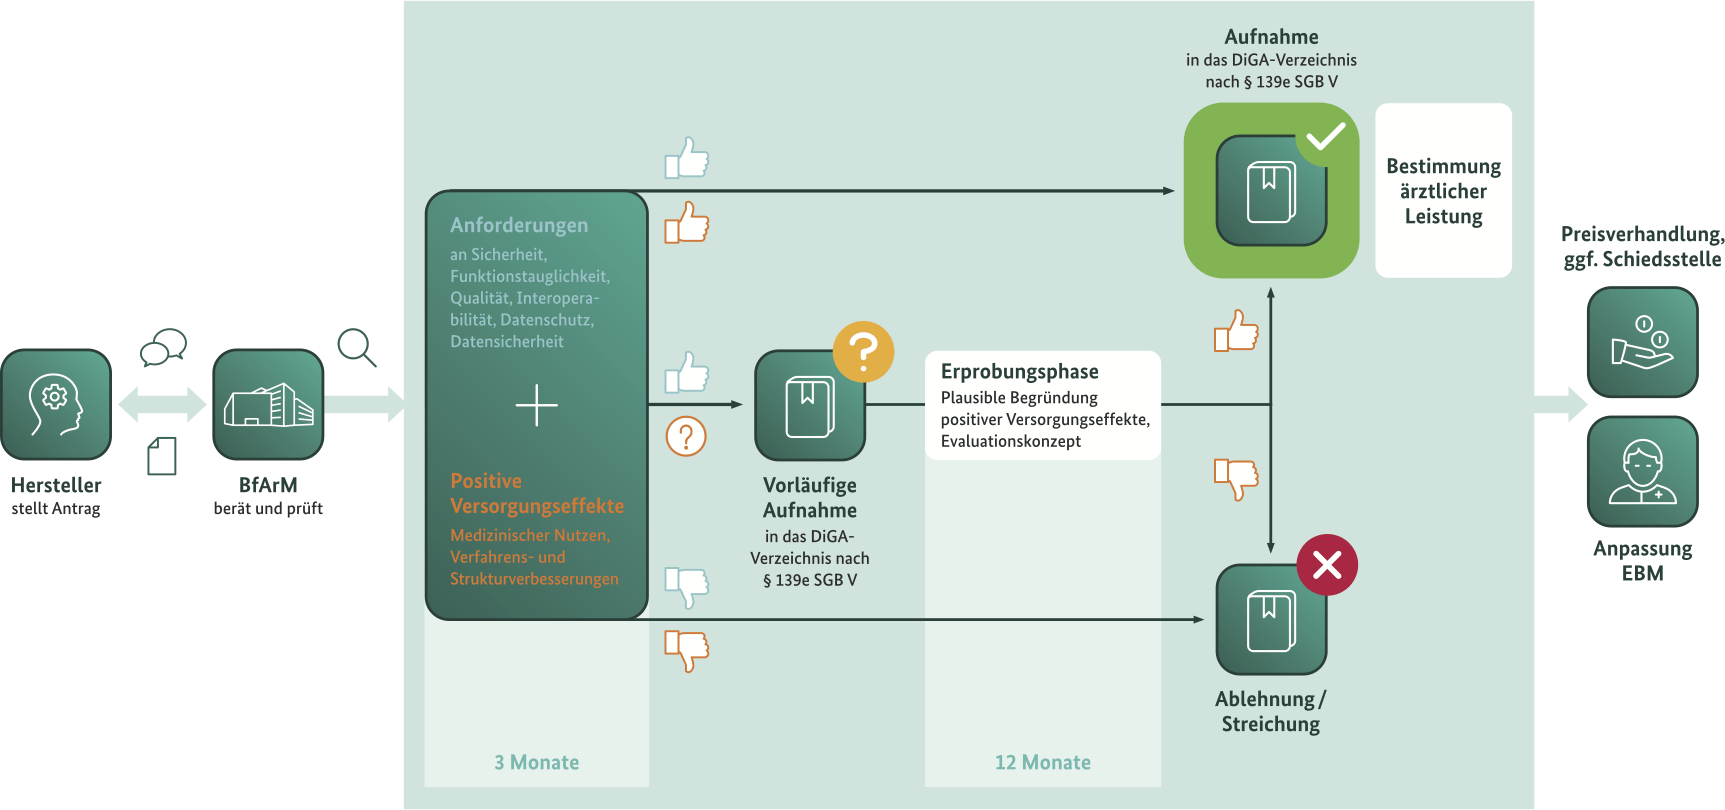
\includegraphics[width=\textwidth]{./grafiken/fast-track-verfahren}
				\caption[Ablaufdiagramm des Fast-Track-Verfahren]{Ablaufdiagramm des Fast-Track-Verfahren}
			\end{figure}
			Im Türkisen Bereich der Abbildung sieht man, wie das Fast-Track-Verfahren abläuft. Im grünen Kasten, auf der linken Seite des Türkisen Bereichs, sieht man die 2 Voraussetzungen für eine erfolgreiche Antragsstellung die über 3 Monate hinweg vom Bundesinstitut für Arzneimittel und Medizinprodukte. Dabei gibt es die technischen Anforderungen, wie: Sicherheit, Qualität, Datenschutz etc. und die Positiven Versorgungseffekte: Medizinischer Nutzen, Verfahrens- und Strukturverbesserungen. Sollten beide Voraussetzungen erfüllt sein, wird der Antrag akzeptiert und es kommt zu Preisverhandlungen, wie man rechts oben im Türkisen Bereich sehen kann. Sollten beide Voraussetzungen nicht erfüllt sein, wird der Antrag abgelehnt, wie man rechts unten im Türkisen Bereich sehen kann. Sollten nun die technischen Anforderungen erfüllt sein, aber der Positive Versorgungseffekt noch fragwürdig sein, wird die DiGA vorläufig aufgenommen und es kommt zu einer 12-Monatigen Erprobungsphase.
	\section{Informationen zu den DiGAs}        

\bibliographystyle{plain}
\bibliography{seminar_arbeit_marcelo}
\end{document}